\documentclass[a4paper,12pt]{report}
\usepackage{graphicx}
\usepackage{pgfplots}
\usepackage[strings]{underscore}
\usepackage[T1]{fontenc}
\usepackage{amsmath}
\usepackage[backend=bibtex]{biblatex}
\bibliography{dissertation}

\addtolength{\oddsidemargin}{-.5in}
\addtolength{\evensidemargin}{-.5in}
\addtolength{\textwidth}{1in}

\addtolength{\topmargin}{-.5in}
\addtolength{\textheight}{1in}
\begin{document}
\title{Writing a Program to Evaluate Lambda Expressions}
\author{Yola Jones}
\date{\today}
\maketitle

%
% 	WHAT TENSE IS THIS
%

\chapter{Design and Implementation}
\section{Design}

The overall program is split into a number of distinct elements, all of which are based on the fundamental rules of Lambda Calculus (such as syntax and evaluation rules) as defined previously.\\

Firstly, a grammar is written which defines the syntax of lambda terms and allows a term to be broken down into individual tokens. Antlr uses this grammar to process lambda terms, creating an Abstract Syntax Tree for each incoming expression\cite{Parr2012}, a process which has been well documented and therefore will not need to be rewritten. A tree traversal mechanism is the main section of code which navigates the abstract syntax tree and performs operations to determine the resultant expression. This is the section of code which will perform the evaluation, and therefore needs to be designed effectively, with the rules of beta reduction and lambda calculus in mind. A web interface is used to house this program, giving the user a simple and convenient way to interact with the underlying system.\\

The relevant sections have been discussed below, detailing design and key decisions which needed to be made before implementation began. %WHAT TENSE IS THIS

\subsection{Grammar}

The key aim in creating this grammar was creating a syntax which sticks as closely as possible to the rules of lambda calculus. Lambda Calculus grammar is already clearly defined, with a lambda term being either a variable, an abstraction or an application \cite{Hankin2004}. Applied lambda calculus adds functions and constants to this definition \cite{Slonneger1995}, resulting in the following lambda grammar. A lambda term is one of the following:

\begin{itemize}
\item[|] An application (of form \texttt{[term] [term]})
\item[|] An abstraction (of form \texttt{[abstraction_term].[term]} where \texttt{[abstraction_term]} is defined by \texttt{$\lambda$[variable]})
\item[|] A function (of form \texttt{[term] [operation] [term]})
\item[|] A value (of form \texttt{[variable]} (the letters a-z) or \texttt{[number]} (constant))
\end{itemize}

With the addition of types, the grammar adds the option of a \texttt{:[type]} term to each variable, with each type being either a ground type (bool, int or none), or in the form \texttt{[type]->[type]}. This follows the standard syntax for typing used in the lecture material \cite{Hankin2004} \cite{Gay2019}, and will allow students on the Theory of Computation course to input a lambda term directly from the lecture slides with minimal adjustment.

\subsection{Expression Evaluator}

The fundamental component of this evaluator is a tree traversal, which navigates through the token nodes and performs different operations depending on the type of node encountered. For example, application tokens in the form MN will pass the right-hand term N to the left-hand term M. Abstractions will take an incoming value if one exists, and substitute it into the body of the abstraction. This will allow an evaluated expression to be built up, and a result determined.\\

Antlr provides two mechanisms for traversing an abstract syntax tree: listeners and visitors. A listener is a passive way of evaluating a syntax tree, used with an antlr Walker which traverses the tree using a depth-first approach, triggering methods from the listener as it enters and exits each token \cite{Parr2012}. These listener methods are unable to return values, so expressions and evaluations have to be handled using separate objects within the listener class. As the walker traverses the tree, the listener builds up a running evaluation of the term, returning the result when it exits the topmost node \cite{Srivastav2017}.\\

Unlike listeners, visitors control their own traversal of the tree. By visiting the children of each node encountered explicitly, the path they take around the tree can be controlled \cite{Parr2012}, allowing some children to not being visited until their parents are evaluated, or a right-hand child of a node being visited and evaluated before its left.\\

Visitors also allow custom return types, meaning nodes can return their resultant expressions directly to their parent node and do not have to rely on separate objects \cite{Srivastav2017}.\\

With beta reduction, different methods take different approaches to evaluating terms. In an application MN using a call-by-value approach, N is evaluated before M. In a call-by-need approach, N is passed into M before being evaluated. This means that depending on the type of reduction selected, the evaluator will have to traverse the tree in a different order, suggesting visitor is more appropriate for this task than a listener. The fact that evaluation happens as the tree is being visited supports this further, since there will be a large amount of data being passed around the tree. Having a separate object for storing these values could get complex, and so the visitor methods being able to return values directly to their parents will be more convenient for this task.\\

The visitor therefore will be the main code written in this project. An Antlr generated parser will be passed to a custom visitor interface. Different visitors will be defined for each of the beta-reduction strategies being implemented, since each method takes a different approach to evaluating expressions.\\

The visitor should return three separate items upon returning to the topmost node: the evaluated value of the input lambda term, whether or not the term is typable, and what type the expression will be. It will also return details of any errors where applicable, for example syntax errors which Antlr can't parses, or cases where the normal form of a lambda term does not exist.

\subsection{Web Interface}

The web interface will allow the user to input a lambda term along with the types of any variable. It will also allow the user to select which reduction strategy they would like to have the term evaluated by, with call-by-need (or normal order reduction) being selected as the default.\\

The code running the interface and the underlying evaluation code will be kept as separate entities, communicating through input parameters and return statements. This is to ensure the code is kept as modular as possible, allowing the evaluator code to be run using multiple different mechanisms, for example through a web interface and a command line for testing purposes. Any data the user enters will be passed to the underlying code, which will process the term and return any output via a return statement, which will be read and displayed to the user.\\

The layout of the interface should be simple and uncluttered, and should be suitable for those with a visual impairment.

\section{Implementation}

The majority of the code has been written in Python, specifically Python3, as there is plenty of support for Antlr being used with Python3. While Java is more extensively supported in Antlr, the MSc Software Development course which this dissertation is being written for teaches Java and not Python, so Python was chosen as a way of expanding the number of programming languages encountered throughout the course.

\subsection{Grammar}

The lambda grammar is contained in a .g4 file which defines the parser and lexer rules for lambda calculus, as required by Antlr. A section of the grammar is shown in \ref{parser_rules}, and indicates the parser rules for the term, application and abstraction token nodes, alongside the lexer rules in \ref{lexer_rules}.

\begin{figure}[p]
\centering
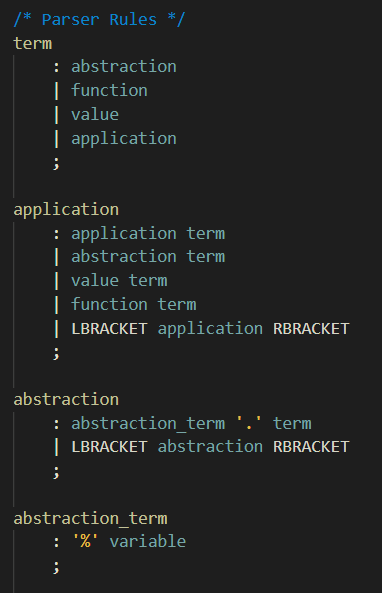
\includegraphics[scale=0.75]{images/parser_rules}
\caption{Parser Rules}
\label{parser_rules}
\end{figure}

\begin{figure}[p]
\centering
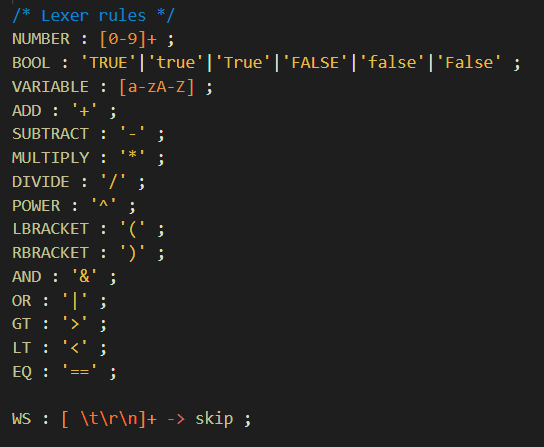
\includegraphics[scale=0.75]{images/lexer_rules}
\caption{Lexer Rules}
\label{lexer_rules}
\end{figure}

\subsection{Abstract Syntax Tree}

Having defined a grammar, antlr can then be used to create an abstract syntax tree. This is very simple to do, and involves passing the input term through an Input Stream class which converts this to a string of characters, then feeding this into a lexer (which outputs a set of tokens), a class which converts the tokens into an indexable list, and finally passing this through a parser which turns the tokens into an abstract syntax tree which can be explored \cite{Tomassetti2007}. This process is well documented and therefore will not be deviated from.\\
%screenshots needed here

\subsection{Expression Evaluator}
This is the largest block of code in the program, and defines how the incoming lambda term should be evaluated depending on the input given by the user. This code can be split into three distinct sections as discussed in the Background chapter of this report: alpha conversion, beta reduction and typing rules.

\subsubsection{Alpha Conversion}
The alpha conversion is based on the rules for explicit alpha conversion with substitution, as defined by \cite{Acar2008}, and as discussed in detail previously. These rules are as follows:

\begin{equation}
[t/x]y=\begin{cases}
t & \text{if $y=x$}\\
y & \text{if $y\ne x$}
\end{cases}
\end{equation}

\begin{equation}
[t/x](t_1t_2)=[t/x]t_1[t/x]t_2
\end{equation}

\begin{equation}
[t'/x](\lambda y.t)=\begin{cases}
\lambda y.t & \text{if $x=y$}\\
\lambda z.[t'/x][z/y]t & \text{if $x\ne y \land z\notin FV(t) \cup FV(t')$}
\end{cases}
\end{equation}

The final rule is the rule to be focused on, and contains the process of finding a variable z that does not appear in the free variables of the incoming term or the existing term, replacing all bound variables y with this new term z, and then substituting in t’ as normal.
The alpha conversion code follows this process. First, the set of free variables in the term are determined, by taking the set of all alphabetic characters in the term and eliminating the bound variables. These variables are then replaced with letters that are not in the list of free variables, in the situation where a clash in free variables between the two expressions are found. This produces an alpha-converted term, and regular substitution happens using a string.replace() python method, as abiding by the Barendregt Convention.

\subsubsection{Beta Reduction}

Two beta reduction strategies are taught on the Theory of Computation course, call-by-value and call-by-name. The differences between these two strategies have been discussed, but the key difference is in when terms are evaluated in an application MN, whether N is evaluated before being passed into M, or whether it is substituted first and then evaluated inside M.\\

Because of these differences in evaluation strategy, two separate visitors are used. However, since they share a lot of the same common functionality (when alpha conversion happens, typing rules, what happens inside functions), a BaseVisitor was defined which contains all common code between these two strategies. The two call-by-value and call-by-need visitors are subclassed from this base visitor, and define their unique behaviour for the application and abstraction terms.\\

The abstraction term differs between the two methods due to nothing other than typing, since the type of a term happens during the evaluation of that term as will be discussed in more detail below. In call-by-value, the type of N is known before substitution, so can be carried throughout the function. In call-by-need, the whole term needs to be type checked after substitution has happened to determine the type of M with N incorporated.

\subsubsection{Typing}

Lambda Calculus has clearly defined typing rules which are taught in the Theory of Computation course. These rules have been discussed in more detail previously, and are as follows:

\begin{equation}
\frac{x:T\in \Gamma}{\Gamma \vdash x:T}TVar
\label{variable_type}
\end{equation}

\begin{equation}
\frac{\Gamma ,x:T\vdash M:U}{\Gamma \vdash \lambda x:T.M:T \to U}TAbs
\end{equation}

\begin{equation}
\frac{\Gamma \vdash M:T \to U \qquad \Gamma \vdash N:T}{\Gamma \vdash MN:U}TApp
\label{application_types}
\end{equation}

There are two minimal types (\texttt{int} and \texttt{bool}) and one supertype (\texttt{none}) as defined in the Theory of Computation lecture slides \cite{Gay2019}. These will be the only types allowed by the program.\\

Since the visitNode methods already evaluate their children nodes, these typing rules can be integrated directly into these nodes, with each visitNode method returning a value and a type. Type checking happens throughout the code, in each method which could contain conflicting types. This is implemented as follows:\\

\textit{Abstraction}\\
Users enter types in the form \texttt{x:type}, which can be applied to any variable included in the term. This means that the term \texttt{$\lambda$ x:int.x:bool} is valid, but type invalid (since the type of x is different for each x term). This is checked inside the visitAbstraction method.

The abstraction method takes the input type T (as determined either from input by the user or through type inference from a function, discussed below), and joins it with the output type (again, either from user input or determined from the function) with \texttt{->}, to become of type \texttt{input->output}.\\

\textit{Application}\\
Application typing is far simpler than abstraction, for an application MN the code simply takes the type of M (in the form \texttt{T} or \texttt{T->U}) and iteratively removes the first type from both M and N until the type of N is None, at which point it returns type M. If at any point the first type in M does not match the first types in N, or the number of types in N is larger than the type of M, the type checking is declared invalid. This is as per rule \ref{application_types}.\\

\textit{Variable}\\
The variable terms return the type given to them by the user, as defined by Rule \ref{variable_type}. Any number is given type \texttt{int}, and any boolean values TRUE or FALSE are given type \texttt{bool}.\\

In the visitFunction node, the input and output types of terms can be inferred by examining the operation term. The following is stated in code:

\begin{itemize}
	\item The operations \{\&,|\} take two boolean values and return a boolean. Therefore the type of the incoming term can be inferred to be a bool, likewise with the output term
	\item The operations \{+,-,*\} take two integer values and return an integer. As above, the input term can be inferred to be an integer, matching the output term
	\item The operations \{==,>,<\} take two integer values and return a boolean, so it can be inferred that the input term is an integer, and the output is a boolean. 
\end{itemize}

This is used to determine the output type of a function which is used to determine the type output by its parent term. In an abstraction, this type inference can be used to determine the type of its input term, for example the lambda term $\lambda x.x+1$ can be inferred to have type \texttt{int->int} despite no input type given by the user.\\

There is a limit to this type inference, the function will infer the input type when there is only one operation term. For example, the term $\lambda x.(x==1)\&b$ contains two operations, == and \&. In this case, working out the input type is more complicated, since the typing has to be broken down in to sub-functions, which need to determine what they think the input type should be, which then needs to be examined collectively as a complete term. The type of this output is returned by the program therefore as \texttt{None->bool}, which is correct, it's just not as refined as \texttt{int->bool}.\\

While this is definitely possible, it is not the key goal in the project, and is a small edge-case when it comes to improving students understanding. The result is correct, just not completely minimal. Because of this, and due to the finite nature of this project, this has been deemed an acceptable limitation of the code, with other tasks which more greatly contribute to students understanding of lambda calculus being prioritised.

\subsubsection{Overall Lambda Code}
Each visit method in the visitor returns an evaluated result and a type, which is used to build the evaluated term and determine the final result, type and type validity of the input expression.\\

However, during this process, there are a number of occurrences which could stop the program from being able to return a final result. These are broken down into two key issues: syntax errors and occurrences where a term doesn't have a normal form and therefore cannot be evaluated to termination. These have been discussed below.\\

\textit{Syntax Errors}\\
Lambda terms often include nested parentheses. It is easy for a user to mismatch brackets, for example for a term to include three open brackets but only two close brackets. Because of this, before the term is passed to antlr, the code checks to ensure brackets are matched correctly, and if not, returns an error to the user informing them of the issue and asking them to re-enter.

Apart from this, general syntax errors are likely to occur, for example a user forgetting to put a . in an abstraction term. To handle this, antlr's ErrorListener class is overridden, instead throwing a custom SyntaxTokenError exception, which can be caught by the program and passed back to the user.\\

\textit{Recursion Errors}\\
Recursion errors are thrown in Python when a maximum stack depth is reached in order to protect Python from crashing \cite{PythonStack2019}. This is the exception which is thrown when a lambda term has no normal form, as the code keeps trying to evaluate it before eventually throwing a RecursionError.\\

To handle this, the recursion limit for the code is set to 200, smaller than the python default to prevent excessive time waiting for the program to fail, but large enough to ensure that any reasonable lambda term a student could want to input can be processed. A recursion limit for the code equates to a lambda term with approximately 50 nested abstractions (since each abstraction could potentially be comprised of the following nodes: its parent term, the abstraction contained within parentheses, the actual abstraction and its inner terms). While this is a limitation, it's is deemed to be a reasonable one.\\

If a recursion error is thrown, it is caught by the code in a \texttt{try/except} block, and an error message informing the user that a normal form cannot be found for this term is given to the user.

\subsubsection{Web Interface}

Flask is a web framework designed for use with Python, and allows python scripts to be controlled and run from a web interface which is served by Flask\cite{FullStack2019}. The front-end of the web interface is written in HTML, and is connected to the python file using Flask's render_template() function.\\

Users enter lambda terms in the input dialogue box, and enter the lambda symbol by entering a \texttt{\%} sign. Using a HTML onkeydown event, the interface automatically changes this symbol to a $\lambda$, allowing users to easily enter lambda terms. The complete web interface can be seen in \ref{web_interface_no_input} and \ref{web_interface_input}.\\

Clicking the \textit{Check Expression} button on the web interface sends a HTTP post request to the Flask server, which takes the value held in the user input box along with the selection of reduction strategy, and sends this to the main antlr Lambda program. The result outputted is then given to the HTML code, and the webpage is re-rendered to display the results, be that an error message indicating a syntax or normal form not found error, or the result, type and type validity of the lambda term input by the user.

\begin{figure}[p]
	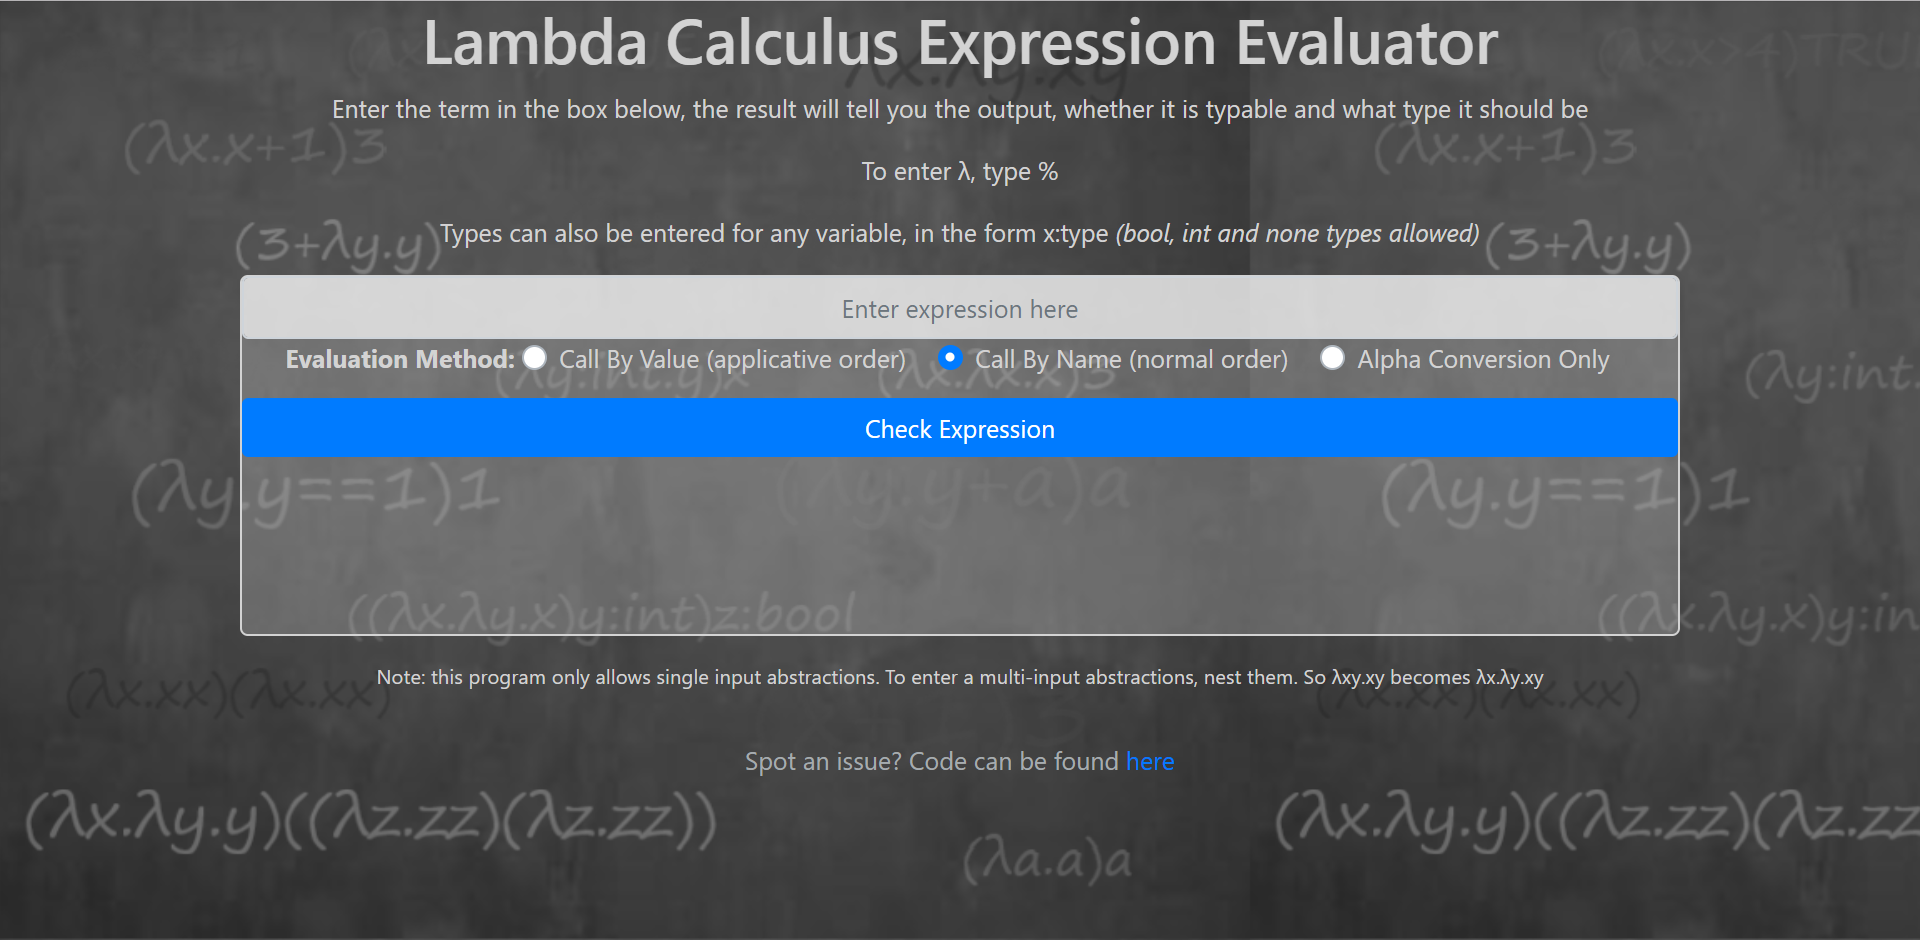
\includegraphics[scale=0.4]{images/web_interface_no_input}
	\centering
	\caption{Web Interface}
	\label{web_interface_no_input}
\end{figure}

\begin{figure}[p]
	\centering
	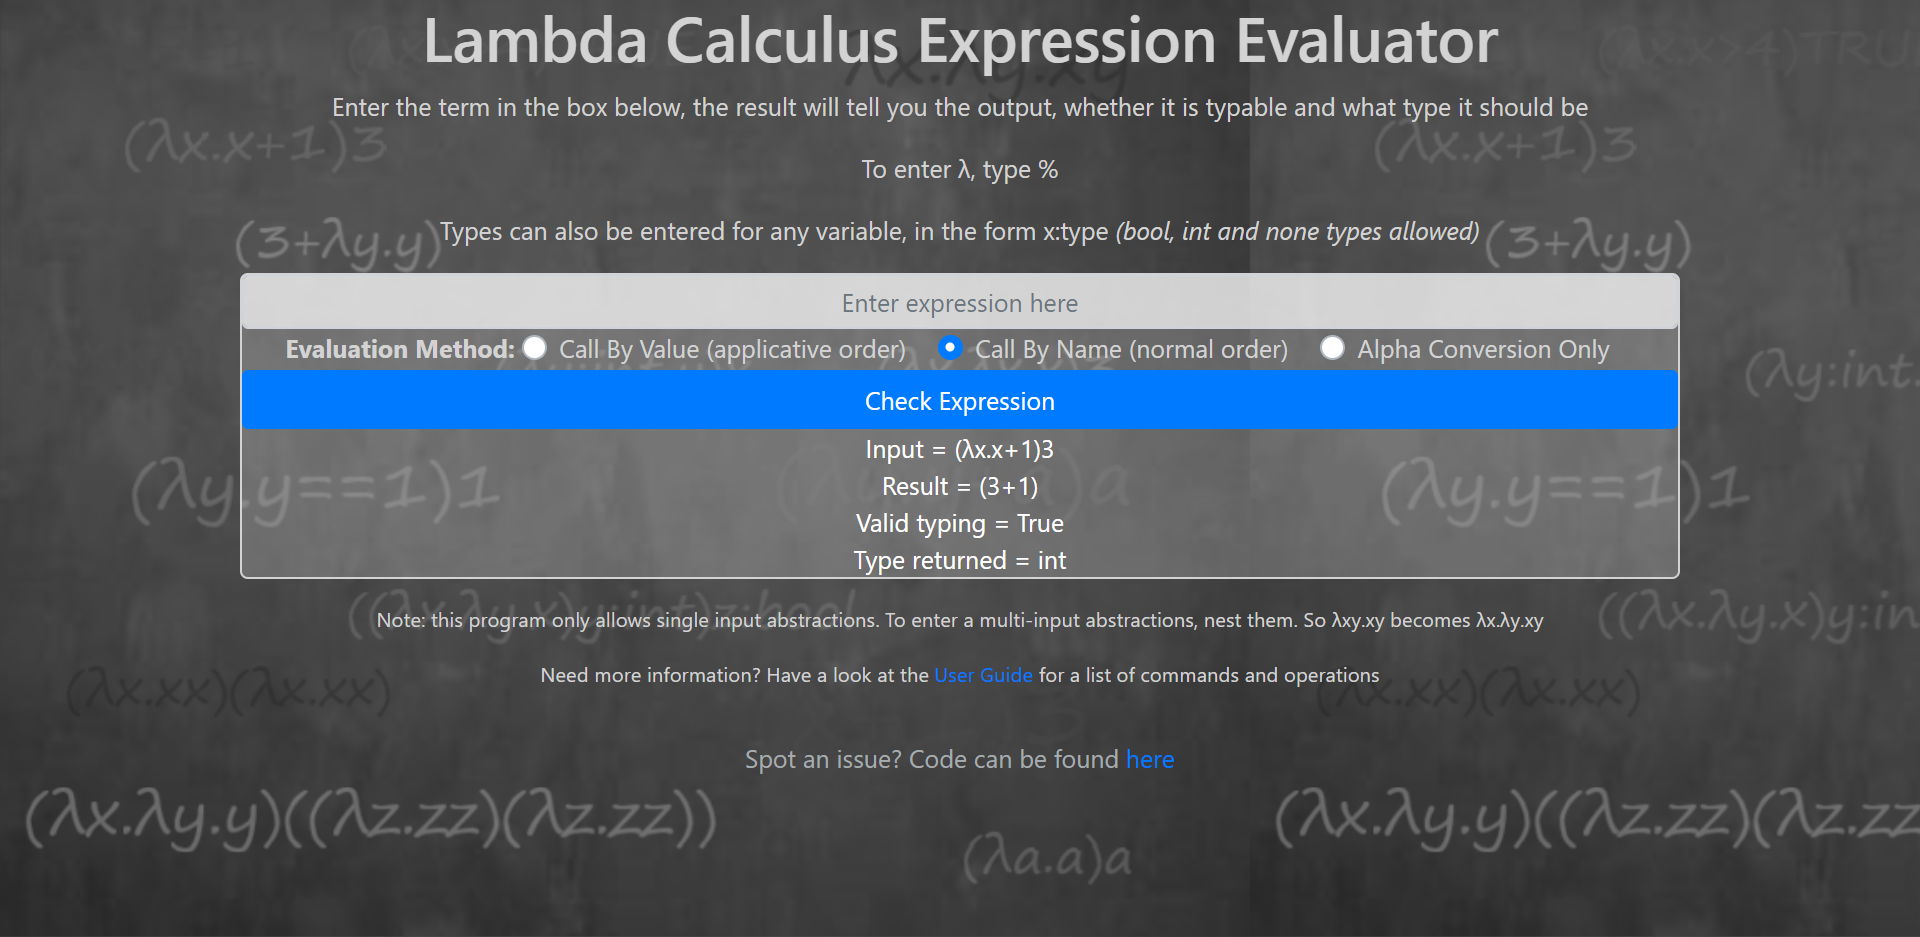
\includegraphics[scale=0.4]{images/web_interface_input}
	\caption{Web Interface With Returned Result}
	\label{web_interface_input}
\end{figure}

\chapter{Testing}
The aim of this project is to build a web application which will verify and evaluate lambda calculus terms input by the user, with the goal of helping future students learning functional programming to gain a better understanding of lambda calculus.\\

This can be broken down into two key goals for the created tool:
\begin{itemize}
	\item The interface should evaluate lambda terms accurately
	\item The interface should be easy to use and understand
\end{itemize}

Because of this, the testing will be broken down into two sections in accordance with these two goals. The first set of tests will evaluate the accuracy of the lambda term evaluation. The second set of tests will test the usability of the interface and whether or not it meets the goal of improving student understanding, by performing a user test with students who have an understanding of computer science but who have little to no knowledge of lambda calculus.

\section{Accuracy of Lambda Term Evaluation}
A page here testing different lambda terms, including:
\begin{itemize}
	\item Alpha conversion
	\item Basic lambda terms
	\item Multi-input lambda terms
	\item Call by value and call by need (with ($\lambda$x.$\lambda$y.y)(($\lambda$z.zz)($\lambda$z.zz)))
	\item Types
	\item Type inference
\end{itemize}
\newpage

\section{Interface Usefulness and Usability}
\label{interface usefulness and usability}
\subsection{Testing}

In order to test the usability and usefulness of the interface, a user test was conducted using participants who had a background in computer science but who had little to no understanding of lambda calculus, in order to simulate students on the Theory of Computation course who have just been introduced to Lambda Calculus for the first time.\\

Participants were first given a Participant Information sheet and to sign a Participant Consent Form, which stated they were happy with the results of the user test to be included in this dissertation, with the confirmation that their answers will be kept anonymous.\\

They were then asked to read a document giving them a brief introduction to lambda calculus, which was written for this test and was based on the Theory of Computation lecture slides \cite{Gay2019}. (should I put this document in the appendix?) This was done in order to give them a small introduction, to simulate students who have attended a couple of lectures in lambda calculus and therefore have a slight starting point, but are still very new to the subject.\\

They were then asked to rate their understanding of lambda calculus on a scale of 1-10, before being given the interface to test. They were also provided with a few sample lambda terms to test if they wanted to, but were not obligated to use. This was to simulate students who may be using the tool to evaluate a particular lambda expression they have found in the lecture slides or online.\\

Although the test was not conducted with a time limit, each participant spent approximately five minutes using the interface before stating they were ready to move on.\\

Finally, users were given a questionnaire which again asked them to rate their understanding of lambda calculus having used the interface for a short period of time, so their understanding could be compared before and after using the tool.\\

The questionnaire also asked the following questions:
\begin{itemize}
	\item Would you use a tool like this if you were studying the Theory of Computation Course?
	\subitem Yes/no/other (please detail...)
	\item Did you find it useful in improving your understanding?
	\subitem Yes/no/other (please detail...)
	\item What did you think of the interface?
	\item Do you have suggestions for any improvements that could be made?
	\item Any further comments?
\end{itemize}

\subsection{Results}
As can be seen from figure \ref{participant_understanding}, in the 5 minutes participants interacted with the interface, their understanding improved by 15\% on average. 100\% of participants said they would use the tool created if they were on the Theory of Computation course, and 100\% said they found it useful in improving their understanding.\\

The qualitative questions on the interface and tool revealed that participants found the system simple and easy to use, with suggestions for improvement including adding tooltips to give the user more information, and changing the colour of the input box to make it more obvious that it is an input box and not a menu.\\

Overall the feedback was incredibly positive, supporting the conjecture that the tool created could support student learning for those learning lambda calculus for the first time.\\

[I am going to add more participant data to this - so far I have done two user tests, I'm expecting 4 more]

[Note to self: should I include the results from the google survey in the appendix?]

\begin{figure}[h]
	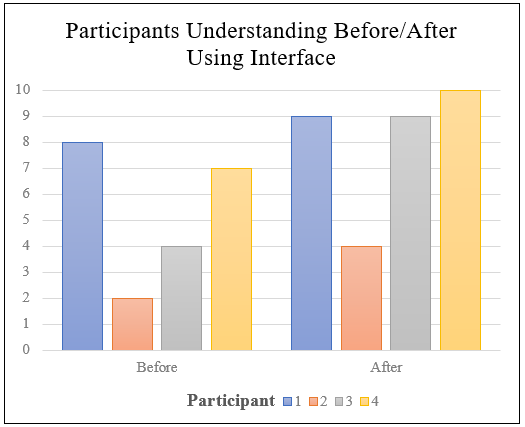
\includegraphics{images/participant_understanding}
	\centering
	\caption{Participant Understanding Results}
	\label{participant_understanding}
\end{figure}

\chapter{Evaluation}

As stated in the beginning of this report, the project summary is as follows:

\begin{quote}
	 \textit{The aim of this project is to build a web application which will verify and evaluate lambda calculus terms input by the user. This tool will be created with the goal of helping future students learning functional programming to gain a better understanding of lambda calculus.}
\end{quote}

This chapter will discuss whether or not the project description has been met, and whether or not the tool created could be used as a supplementary resource for students learning lambda calculus on the Theory of Computation course taught at the University of Glasgow.

\section{Accurately Evaluating Lambda Terms}
As evidenced by the [software testing] section of this report, the tool created does accurately evaluate lambda terms, returning the normal form, type and type validity of lambda terms for both call-by-value and call-by-need evaluation strategies. Applied lambda calculus with types is supported, as taught on the Theory of Computation Course.\\

[list of known limitations and bugs]
[limitations: mutual left recursion issue (discuss in Future Work), type inference]

\section{Improving Student Understanding}
The user tests conducted and summarised in the \ref{interface usefulness and usability} section of this report suggest that students with a computer science background learning lambda calculus for the first time would likely find the tool useful in supporting their learning. Possible improvements such as including tooltips as suggested in user feedback are valid and would be implemented given more time.\\

The user feedback also suggested that the simplicity of the interface is a positive, and care must be taken to prevent the interface from becoming too complicated. The interface is to be used as support for the Theory of Computation lecture slides or other lambda calculus guidance, as opposed to teaching those using the interface lambda calculus.\\

With a goal of supporting learning by providing an interface which accurately evaluates lambda terms, it can be said that these goals have been met.\\

\section{Future Work}
Due to the time limited nature of this project, not all features or corrections have been implemented. Given more time, the following work would be done:

\begin{enumerate}
	\item Fix the bugs discussed previously
	\item Add in multi-input abstraction terms to allow users to enter $\lambda xy.M$ as appears in the lecture slides \cite{Gay2019} as opposed to $\lambda y.\lambda y.M$
	\item Improve the type inference to allow input types of multi-operation functions to be inferred
	\item Include tooltips linked to various aspects of the web interface to give users more information
	\item Do further user testing for the web interface to get a wider understanding of any style/usability issues that exist 
	\item Allow users to enter lambda terms in the De Bruijn notation, for those unfamiliar with the Barendregt convention
\end{enumerate}

\printbibliography

\end{document}